% Great thanks for Cezary Sałbut (this latex file is mainly based on his work)

\documentclass[a4paper,12pt,fleqn]{article}


\usepackage[utf8]{inputenc} 
\usepackage{polski}
\usepackage[polish]{babel}
\usepackage[pdftex]{color,graphicx}
\usepackage{subfig}
\usepackage{indentfirst}
\usepackage{booktabs}
\usepackage{tabularx}
\usepackage{multirow}
\usepackage{pdflscape}
\usepackage{array}
\usepackage{amsmath}
\usepackage{appendix}
\usepackage{hyperref}
\hypersetup{
    colorlinks,%
    citecolor=black,%
    filecolor=black,%
    linkcolor=black,%
    urlcolor=blue
}

\usepackage{listings}
\lstset{
	numbers=left, 
	stepnumber=1, 
	basicstyle={\footnotesize \ttfamily},
	language=C, 
	captionpos=b,
	xleftmargin=6mm,
	aboveskip=\medskipamount,
	belowskip=\bigskipamount,
	tabsize=4
}

\usepackage{title-page}

\usepackage[top=28mm, bottom=30mm, left=21mm, right=21mm]{geometry}

\linespread{1.5}		%interlinia

\usepackage{boxedminipage} 
%% change the below lengths to suit your needs: 
\setlength{\fboxrule}{1pt} 
\setlength{\fboxsep}{5pt}



\renewcommand{\appendixtocname}{Dodatki}
\renewcommand{\appendixpagename}{Dodatki}


\widowpenalty=10000
\clubpenalty=10000


\newcommand{\autor}{Jan Kurdel}
\newcommand{\tytulpl}{Identyfikacja nieliniowych obiektów dynamicznych metodą uogólnionej regresji postępującej z ortogonalizacją}
\newcommand{\tytulen}{Identification of nonlinear dynamical objects based on Generalized Orthogonal Forward Regression}
\newcommand{\uczelnia}{POLITECHNIKA WARSZAWSKA}
\newcommand{\wydzial}{Wydział Elektroniki i Technik Informacyjnych}
\newcommand{\instytut}{Instytut Systemów Elektronicznych}
\newcommand{\promotor}{dr inż. Stanisława Jankowskiego}
\newcommand{\praca}{Praca inżynierska}
\newcommand{\miejscerok}{Warszawa, 2012}
\newcommand{\indeks}{214460}

\title{\tytulpl}
\author{\autor}

\begin{document}

\renewcommand{\tablename}{Tabela}

\pagestyle{empty}
\stronatytulowa

\newpage
\setcounter{page}{1}

\newpage
\textbf{\tytulpl} \vspace*{0.2cm} \\
Praca opisuje identyfikację obiektów dynamicznych metodą uogólnionej postępującej regresji ortogonalnej. W pracy została przedstawiona identyfikacja obiektu opisanego równaniem Van der Pola. Następnie została oceniona jakość zidentyfikowanego modelu poprzez predykcję z wykorzystaniem tego modelu.

\vspace*{2cm}
\textbf{\tytulen} \vspace*{0.2cm} \\
The object of the thesis is identification of nonlinear dynamical objects based on Generalized Orthogonal Forward Regression. This aim was realized based on object described by Van der Pol differential equation. After that quality of model was evaluted by prediction with use of this model. 

\newpage
\tableofcontents

\newpage
\pagestyle{plain}

\section{Cel pracy}
Praca ma na celu identyfikację nieliniowych obiektów dynamicznych z wykorzystaniem metody GOFR. W pracy zostanie przestawiona próba predykcji modelu opisanego równaniem różniczkowym Van der Pola na minimum kilka kroków w przód. Następnie zostania ocenione jakość predykcji jak również sama metoda uogólnionej postępującej regresji ortogonalnej.  Taka predykcja może mieć zastosowanie w wielu zagadnieniach rzeczywistych. 

\newpage
\section{Dynamika obiektów}
Układ dynamiczny to matematyczny model, który opisuje ewolucję realnego zjawiska. Model taki pozwala na analizę reakcji badanego obiektu na pojawiające się zmiany.
Układ dynamiczny z czasem ciągłym jest opisywany układem równań ruchu w postaci ogólnej\cite{Kosinski}
\begin{equation}
	\frac{dx}{dt} = F(x,r), \quad x \in R
\end{equation}

gdzie: \\
$F$ - odwzorowanie $F:U \rightarrow R^n$,
$r$ - zbiór parametrów kontrolnych układu,
$U$ – podzbiór $R^n$ określający przestrzeń fazową układu.

Przestrzeń fazowa jest przestrzenią wszystkich możliwych stanów w jakich może znajdować się badany układ. Każdy stan układu jest pojedynczym punktem tej przestrzeni.
Aby określić ewolucję czasową układu należy scałkować równania ruch układu w pewnym przedziale czasu $\delta t$. Otrzymana w ten sposób rodzina funkcji $\phi_i(t,r)$ jest nazywana strumieniem. Konkretne rozwiązanie układu równań ruchu $\phi_i(t_0,r)$ - dla danych wartości parametrów $r$ i warunków początkowych zwane jest orbitą (trajektorią).

Jeśli odwzorowanie $F$ jest odwzorowaniem liniowym to układ dynamiczny jest układem liniowym, natomiast jeśli $F$ jest odwzorowaniem nieliniowym to układ dynamiczny nazywamy układem nieliniowym.

Uniwersalnym sposobem opisu dynamiki obiektów z czasem ciągłym są równania różniczkowe. Dla opisu dynamiki obiektów z czasem dyskretnym odpowiednio stosowane są równania różnicowe\cite{Gutenbaum}[str. 73].
\subsection{Równania różniczkowe zwyczajne}

Równaniem różniczkowym zwyczajnym nazywamy równanie zawierające zmienną niezależną $x$, nieznaną funkcję $y$, oraz jej pochodne $y', y'', \hdots, y^{(n)}$ \cite[str. 7]{BCh_2001}
\begin{equation}
	\label{wzor:rownanie_roz_N_stopnia}
	F(x,y,y',\hdots,y^{(n)}) = 0
\end{equation}
gdzie $F:R^{n+2} \rightarrow R$

Warunek początkowy (Cauchy'ego) dla równania \ref{wzor:rownanie_roz_N_stopnia} określony jest poprzez: 

\begin{equation}
\begin{array}{c}
y(x_0)       =  y_0,     \\
y'(x_0)      =  y_1,     \\
\vdots			   	     \\
y^{n-1}(x_0) = y_{n-1}
\end{array}
\end{equation}
gdzie $y_0, y_1, \hdots, y_{n-1}$ są zadanymi liczbami.

Stopień pochodnej w równaniu \ref{wzor:rownanie_roz_N_stopnia} decyduje o rzędzie równania różniczkowego. Równanie różniczkowe pierwszego rzędu wyraża się zatem wzorem:
\begin{equation}
	\label{wzor:rownanie_roz_I_stopnia}
	y' = f(x,y)
\end{equation}

Rozwiązanie równania \ref{wzor:rownanie_roz_I_stopnia} w sposób numeryczny może zostać rozwiązane z wykorzystaniem wielu sposobów. Można wyróżnić podział na metody jednokrokowe, które wymagają jedynie informacji z poprzedniego kroku (zatem warunek początkowy jest wystarczający do obliczenia równania różniczkowego dla kolejnego punktu) oraz metody wielokrokowe, w których rozwiązanie jest dokonowywane z wykorzystaniem znajomości kilku poprzednich kroków. Wśród metod jednokrokowych znajdują się m.in. metody Eulera oraz Rungego-Kutty.

\subsection{Metody rozwiązywania równań różniczkowych}

\subsection*{Metoda Eulera}
Metoda Eulera jest najprostszą metodą numeryczną rozwiązywania równań różniczkowych. Mając dane równanie \ref{wzor:rownanie_roz_I_stopnia} oraz warunek początkowy postaci:
\begin{equation}
	y(x_0) = y_0	
\end{equation}
poszukujemy rozwiązania dla kolejnego momentu $x_1 = x_0 + h$ gdzie $h$ jest krokiem metody. W tym celu możemy skorzystać z rozwinięcia szeregu Taylora w pobliżu punktu początkowego $x_0$:
\begin{equation}
	y(x_0 + h) = y(x_0) + hy'(x_0) + \frac{h^2}{2!}y''(x_0) + \hdots
\end{equation}
Korzystając tylko z dwóch pierwszych elementów szeregu Taylora otrzymamy:
\begin{equation}
	y(x_0 + h) = y(x_0) + hy'(x_0) = y(x_0) + hf(x_0,y_0)
\end{equation}
Powtarzając tę czynność wielokrotnie otrzymamy wzór:
\begin{equation}
	y_{n+1} = y_{n} + hf(x_n,y_n)
\end{equation}
określany jawną metodą Eulera.

\subsection*{Metoda Rungego-Kutty}
Kolejną metodą numerycznego rozwiązywania równań różniczkowych jest metoda Rungego-Kutty, która jest metodą wieloetapową. W każdym kroku konieczne jest obliczenie wartości funkcji $f$ dla różnych argumentów. Wśród metod Runge-Kutty można wyróżnić różne metody w zależności od rzędu metody. Najprostszą z nich jest metoda Runge-Kutty rzędu II. Przyjmuje ona postać:
\begin{equation}
	y_{i+1} = y_i + \frac{h}{2}(k_1 + k_2)
\end{equation}
gdzie
$$\begin{array}{c}
	k_1 = f(t_i,y_i) \\
	k_2 = f(t_i + h, y_i + hk_1)
\end{array}$$

Najbardziej popularną jest metoda rzędu IV, która przyjmuje postać:
\begin{equation}
	y_{i+1} = y_i + \frac{h}{6}(k_1 + 2k_2 + 2k_3 + k_4)
\end{equation}
gdzie
$$\begin{array}{c}
	k_1 = f(t_i,y_i) \\
	k_2 = f(t_i + \frac{h}{2}, y_i + \frac{h}{2}k_1) \\
	k_3 = f(t_i + \frac{h}{2}, y_i + \frac{h}{2}k_2) \\
	k_4 = f(t_i + h,y_i + hk_3) \\
\end{array}$$

\subsection*{Równania różniczkowe zwyczajne wyższych rzędów}
Równanie różniczkowe wyższych rzędów może zostać sprowadzone do układu równań różniczkowych rzędu pierwszego \cite[str. 293]{AK_RBG2002}. Mając dane równanie różniczkowego n-tego rzędu:
$$y^{(n)}(t) = f(t,y(t),y'(t),\hdots,y^{(n-1)}(t)), \qquad a \leq t \leq b$$
z warunkiem początkowym w postaci:

$$\begin{array}{c}
y(a)       = \alpha_0,    \\
y'(a)      = \alpha_1,    \\
\vdots					  \\
y^{n-1}(a) = \alpha_{n-1} \\
\end{array}$$

oraz wprowadzając nowe zmienne:
$$y_1(t) = y(t), y_2(t) = y'(t), \hdots, y_n(t) = y^{(n-1)}(t)$$

otrzymujemy układ równań różniczkowych pierwszego rzędu postaci:
$$\begin{array}{l}
y'_1       = y_2   \\
y'_2       = y_3   \\
\vdots			   \\
y'_{n-1} = y_n     \\
y'_n = f(t,y_1,y_2,\hdots,y_n)
\end{array}$$

z warunkami początkowymi postaci:
$$y_1(a) = \alpha_0, y_2(a) = \alpha_1, \hdots, y_n(a) = \alpha_{n-1}$$

Dzięki takiemu zabiegowi możliwe jest rozwiązanie równania różniczkowego wyższego rzędu metodami służącymi do rozwiązywania równań różniczkowych rzędu pierwszego.

\newpage
\section{Sieci neuronowe} 

\subsection{Struktura sieci neuronowych}
Podstawą budowy sieci neuronowych są neurony. Budowa pojedynczego neuronu jest przedstawiona na rysunku \ref{fig:neuron}. Neuron taki sumuje sygnał podany na jego wejścia $x_i$ z odpowiednimi wagami $w_i$, dając na wyjście wynik $y$ sumy przeprowadzonej przez funkcję aktywacji $f(x)$.
\begin{figure}[ht!]
	\centering
	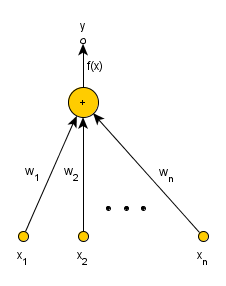
\includegraphics[scale=0.8]{images/single_neuron.png}
	\caption{Budowa pojedynczego neuronu}
	\label{fig:neuron}
\end{figure}

Sieć neuronową budują grupy połączonych ze sobą neuronów. Uproszczoną strukturę sieci wielowarstwowej przedstawia rysunek \ref{fig:multilayer}. Pierwsza warstwa nosi nazwę warstwy wejściowej (\textit{Input}), ostatnia warstwa sieci nosi nazwę warstwy wyjściowej (\textit{Output}). Wszystkie pozostałe warstwy noszą nazwę warstw ukrytych (\textit{Hidden}).

\begin{figure}
	\centering
	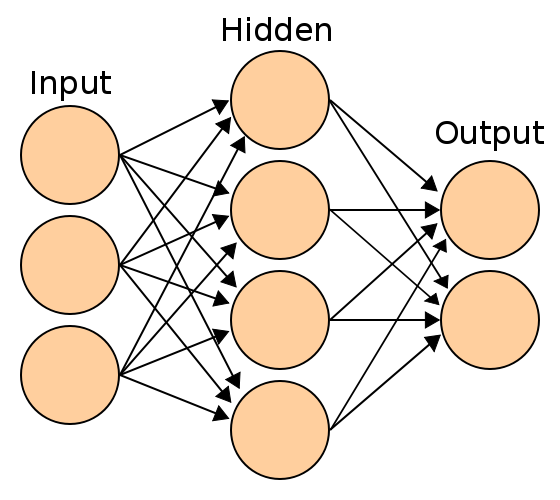
\includegraphics[width=0.5\textwidth]{images/560px-Artificial_neural_network.png}
	\caption{Schemat budowy wielowarstwowej sieci neuronowej}
	\label{fig:multilayer}
\end{figure}

\pagebreak
\subsubsection*{Sieć RBF}
Sieć RBF (Radial Basis Function) jest sztuczną siecią neuronową o radialnych funkcjach bazowych. Sieć taka składa się zazwyczaj z jednej warstwy ukrytej, gdzie funkcja aktywacji jest radialną funkcją bazową oraz 
warstwy wyjściowej w postaci neuronu liniowego. Radialna funkcja bazowa jest określona w sposób następujący\cite[str. 1]{Bartkowiak}
\begin{equation}
	G(x,c) = G(r(x,c))
\end{equation}
gdzie $r(x,c)$ jest odległością między punktami $r$ i $c$ a centrum $c$ jest ustalone i pełni rolę parametru funkcji. Jedną z bardziej popularnych radialnych funkcji bazowych jest funkcja Gaussa:
\begin{equation}
	G(x,\sigma,c) = e^{\frac{-(x-c)^2}{2\sigma^2}}
\end{equation}

\newpage
\subsection{Metody gradientowe uczenia sieci}
Do najbardziej skutecznych metod uczenia sieci neuronowych należą metody gradientowe. Algorytmy te bazują na rozwinięciu w szereg Taylora funkcji celu $E(W)$ w najbliższym sąsiedztwie znanego rozwiązania\cite[str. 54]{Osowski}.
\begin{equation}
	\label{wzor:metoda_gradientowa}
	E(w + p) = E(w) + [(g(w)]^Tp + \frac{1}{2}p^TH(w)p + \hdots
\end{equation}
gdzie
$$g(w) = \nabla E = [\frac{\partial E}{\partial w_1}, \frac{\partial E}{\partial w_2}, \hdots, \frac{\partial E}{\partial w_n}]^T$$
$$H(w) = \begin{bmatrix}
\frac{\partial^2 E}{\partial w_1 \partial w_2} & \hdots & \frac{\partial^2 E}{\partial w_1 \partial w_n}\\
\vdots & & \vdots \\
\frac{\partial^2 E}{\partial w_n \partial w_1} & \hdots & \frac{\partial^2 E}{\partial w_n \partial w_n}
\end{bmatrix}$$
$\nabla E$ jest wektorem pierwszych pochodnych - gradientem, natomiast $H(w)$ jest macierzą drugich pochodnych - hesjanem. W praktyce są używane co najwyżej 3 pierwsze elementy równania~\ref{wzor:metoda_gradientowa}. W metodzie gradientowej poszukuje się minimum funkcji celu poprzez taką aktualizację wektora kierunkowego $p$ oraz kroku $\eta$ dla punktu $w_{k+1} = w_k + \eta_k p_k$ aby prawdziwa była nierówność $E(w_{k+1}) < E(w_k)$.

\subsection*{Algorytm Levenberga-Marquardta}
Podczas gdy wcześniej nie została określona konkretna funkcji celu, tak w przypadku algorytmu Levenberga-Marquardta funkcją celu jest błąd średniokwadratowy (sum-of squares error, Mean Squared Error, MSE)\cite[str. 290]{Bishop}.
\begin{equation}
	\label{wzor:mse}
	E = \frac{1}{2} \sum_{n=1}^N(e_n)^2 = \frac{1}{2} \sum_{n=1}^N(y_n - \tilde{y_n})^2
\end{equation}
gdzie $e_n$ jest błędem n-tego wzorca, $y_n$ n-tym wzorcem, $\tilde{y_n}$ wyjściem sieci dla n-tego wzorca.

Zakładając, że aktualnie jesteśmy w punkcie $w_{i}$ i chcemy przemieścić się do punktu $w_{i+1}$, który jest niedaleko oddalony od $w_{i}$, w celu obliczenia nowej wartości błędu $e$ możemy skorzystać z rozwinięcia w szereg Taylora:
\begin{equation}
	\label{wzor:blad_lm}
	e(w_{i+1}) = e(w_{i}) + Z(w_{i+1} - w_{i})
\end{equation}
gdzie $Z \equiv \nabla e$. Po podstawieniu równania \ref{wzor:blad_lm} do równania \ref{wzor:mse} wzór na błąd średniokwadratowy może zostać zapisany jako:
\begin{equation}
	\label{wzor:mse2}
	E = \frac{1}{2}[e(w_{i}) + Z(w_{i+1} - w_{i})]^2
\end{equation}
Chcą zminimalizować równanie \ref{wzor:mse2} ze względu na zmienną $w_{i+1}$ otrzymujemy wzór:
\begin{equation}
	w_{i+1} = w_{i} - (Z^TZ)^{-1}Z^Te(w_{i})
\end{equation}
Jednak taki sposób obliczania $w_{i+1}$ może powodować, że krok $w_{i+1} - w_{i}$ będzie duży a wtedy liniowa aproksymacja szeregiem Taylora może stać się niedokładna. Z tego powodu algorytm Levenberga-Marquardta korzysta ze zmodyfikowanej funkcji celu w postaci:
\begin{equation}
	\label{wzor:mse_lm}
	E = \frac{1}{2}(e(w_{i}) + Z(w_{i+1} - w_{i}))^2 + \lambda (w_{i+1} - w_{i})^2
\end{equation}
Chcą zminimalizować równanie \ref{wzor:mse_lm} otrzymujemy ostatecznie równanie opisujące sposób obliczania wag w kolejnych iteracjach dla algorytmu Levenberga-Marquardta:
\begin{equation}
	w_{i+1} = w_{i} -(Z^TZ + \lambda I)^{-1}Z^Te(w_{i})
\end{equation}
gdzie $I$ jest macierzą jednostkową. Wartość $\lambda$ zmienia się w trakcie obliczania kolejnych wartości $w_{i+1}$. Jeśli błąd $E$ zmniejsza się wartość $\lambda$ jest zmniejszana o określony współczynnik. W przypadku wzrostu wartości błędu wartość $\lambda$ jest zwiększana o określony współczynnik oraz ponownie przyjmowana jest wartość $w_i$.



\newpage
\section{Selekcja funkcji bazowych oparta o metodę GOFR}

\subsection{Selekcja oparta o ortogonalizację oraz metodę najmniejszych kwadratów}
Jedną z metod selekcji najbardziej znaczących funkcji bazowych jest metoda oparta o metodę najmniejszych kwadratów oraz ortogonalizację \cite{Chen}. Metoda ta umożliwia określenie wkładu każdej funkcji bazowej i wybranie tych najbardziej istotnych. Mając dany wektor wag sieci $w = [w_0, w_1, \hdots, w_K]^T$ oraz wektor danych uczących $d = [d_1, d_2, \hdots, d_p]^T$ można zapisać macierz G w postaci:

\begin{equation}
G = \begin{bmatrix}
\phi_{11} & \phi_{21} & \hdots & \phi_{K1} \\
\phi_{12} & \phi_{22} & \hdots & \phi_{K2} \\
\hdots    & \hdots    & \hdots & \hdots    \\
\phi_{1p} & \phi_{2p} & \hdots & \phi_{Kp}
\end{bmatrix}
\end{equation}

gdzie $\phi_{ji}$ oznacza odpowiedź i-tej funkcji radialnej na j-ty wzorzec uczący. Oznaczając przez $g_i = [g_{i1}, g_{i2}, \hdots, g_{ip}]^T$ odpowiedź i-tej funkcji radialnej na wszystkie wzorce uczące można macierz G przedstawić w postaci:
\begin{equation}G = [g_1, g_2, \hdots, g_K] \end{equation}
Dla takich oznaczeń, dla sieci RBF można zapisać następujące równanie:
\begin{equation}
\label{wzor:ofr_rbf}
d = Gw + e\end
{equation}
gdzie $e$ jest błędem niedopasowania sieci. Ortogonalizacja macierzy G pozwala na określenie osobno wpływu każdej funkcji $g_i$ na wartość części pożądanej energii zdefiniowanej jako $(Gw)^2$ \cite{Osowski}. Dzięki temu możliwa jest selekcja najbardziej istotnych funkcji bazowych oraz znaczne ograniczenie ilości funkcji tworzących sieć. Sama ortogonalizacja może zostać dokonana różnymi metodami z czego często stosowaną jest metoda Grama-Schmidta, gdzie w procesie ortogonalizacji macierzy $G$ powstaje macierz ortogonalna $Q$ oraz macierz trójkątna $A$.
\begin{equation}G = QA\end{equation}
\begin{equation}
A = \begin{bmatrix}
1      & a{12}  & a{13}  & \hdots & a_{1K} \\
0      & 1      & a{23}  & \hdots & a_{2K} \\
\hdots & \hdots & \hdots & \hdots & \hdots \\
0      & 0      & 0      & 0      & 1     
\end{bmatrix}
\end{equation}
Po procesie ortogonalizacji oraz wprowadzając nowe oznaczenie $b = Aw$ można zapisać nową postać równania \ref{wzor:ofr_rbf}:
\begin{equation}
	\label{wzor:ofr_rbf2}
	d = QAw + e = Qb + e
\end{equation}
Rozwiązując równanie \ref{wzor:ofr_rbf2} metodą najmniejszych kwadratów otrzymujemy:
\begin{equation}
	b = (QQ^T)^{-1}Q^Td
\end{equation}
Mając dane $b$ oraz $A$ jesteśmy wstanie określić wektor wag $w = A^{-1}b$.
Jak wspomniano wcześniej wartość pożądana energii jest określona jako $(G^w)^2$. Na tej podstawie można zdefiniować wzór określający udział danej funkcji w ogólnym bilansie energii jako:
\begin{equation}
	\epsilon_i = \frac{b_i^2q_i^Tq_i}{d^Td}
\end{equation}

\subsection{Generalized Orthogonal Forward Regression (GOFR)}
Metoda GOFR jest metodą opartą o metodę OLS \cite{Duboisa}. Modyfikację w stosunku do metody GOFR stanowi optymalizacja dokonywana na etapie selekcji każdej funkcji bazowej. \textbf{Optymalizacja ta polega na minimalizacji...} Porównanie obu metod przedstawia schemat z rysunku \ref{ofr_and_gofr}. Linią przerywaną zaznoczony jest krok specyficzny dla metody GOFR.

\begin{figure}[ht!]
	\centering
	
	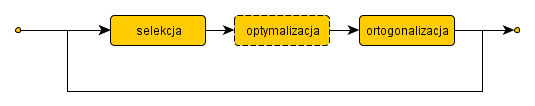
\includegraphics[scale=0.7]{images/ofr_and_gofr.png}
	\caption{Schemat algorytmu OFR oraz GOFR}
	\label{ofr_and_gofr}	

\end{figure}

\clearpage
\section{Identyfikacja systemu opisanego równaniem \mbox{Van der Pola}}

Równanie Van der Pola to równanie różniczkowe wyrażone wzorem:
\begin{equation}
	\label{wzor:van_der_pol}
	y''(t) - (1 - y^2(t))y'(t) + y(t) = 0
\end{equation}
Identyfikację systemu opisanego równaniem \ref{wzor:van_der_pol} oparto o metodę GOFR. W tym celu wygenerowano zbiór danych uczących sieć neuronową rozwiązując równanie metodą Runge-Kutty czwartego rzędu dla warunków początkowych [$y(0)=0,y'(0)=2$], kroku $h=0.1$ w przedziale $t \in [0,50]$. Równanie \ref{wzor:van_der_pol} zapisano w postaci układu dwóch równań różniczkowych pierwszego rzędu:
\begin{equation}
	\begin{array}{l}
    y'(t)  = y_1 \\
    y_1'(t) = (1-y_1^2)y-y_1
    \end{array}
\end{equation}

Powstała w wyniku rozwiązania równania Van der Pola trajektoria, wykres funkcji $y(t)$ oraz jej pierwszej pochodnej $y'(t)$ przedstawione są odpowiednio na rysunkach \ref{img:traj}, \ref{img:func} oraz \ref{img:first_deriv}. Rozwiązanie równania dla przedziału $t \in [0,10]$ zostało odrzucone w celu pominięcia stanów nieustalonych. Rozwiązanie w przedziale $t \in [10,50]$ zostało użyte jako zbiór danych uczących.

\begin{figure}[ht!]
	\centering

	\subfloat[Trajektoria]
	{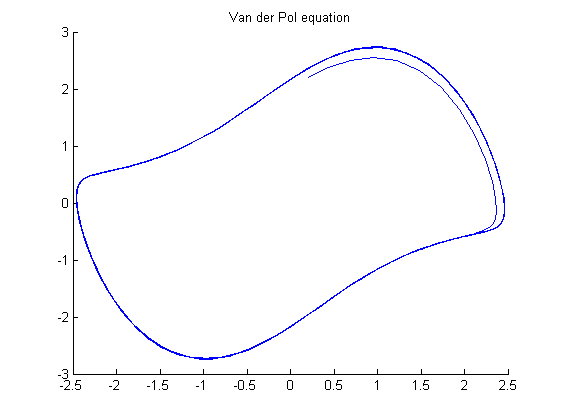
\includegraphics[width=0.5\textwidth]
	{images/trajectory.png}
	\label{img:traj}}
	\subfloat[Wykres funkcji $y(t)$]
	{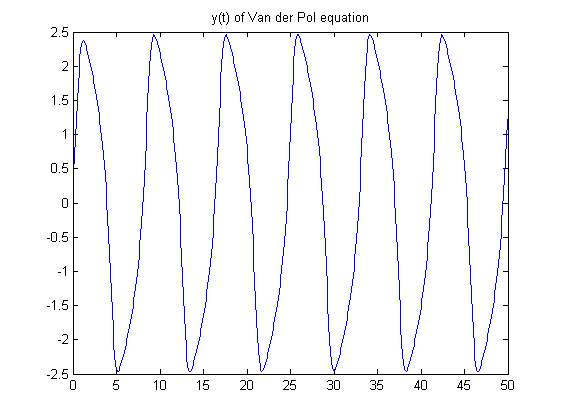
\includegraphics[width=0.5\textwidth]
	{images/signal.png}
	\label{img:func}}
	
	\subfloat[Wykres pierwszej pochodnej $y'(t)$]
	{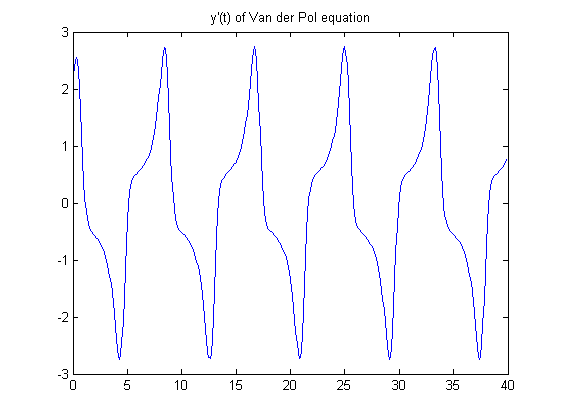
\includegraphics[width=0.5\textwidth]
	{images/first_deriv.png}
	\label{img:first_deriv}}
	
	\caption{Wykresy powstałe w wyniku rozwiązania równania różniczkowego Van der Pola dla warunków początkowych [$y(0)=0,y'(0)=2$]}
\end{figure}

Kolejnym etapem było stworzenie odpowiedniej biblioteki radialnych funkcji bazowych. W tym celu najpierw wygenerowano bibliotekę 115 funkcji RBF postaci:
\begin{equation}
	\label{wzor:rbf_2d}
	f(x_1(t),x_2(t),c_1,c_2,\sigma) = e^{-\frac{(x_1(t)-c_1)^2 + (x_2(t)-c_2)^2}{2 \sigma^2}}\
\end{equation} gdzie: \\
$x_1(t) = y'(t - \Delta t)$ \\
$x_2(t) = y'(t)$ \\

Generowanie biblioteki odbywało się poprzez równomierne dzielenie przestrzeni dwuwymiarowej $D = [min(x_1),max(x_1)] \times [min(x_2),max(x_2)]$. Dla każdego kolejnego poziomu generowania biblioteki funkcji, nowe centra $c_1$ oraz $c_2$ były wybierane poprzez dwukrotnie zagęszczenie punktów w każdej z osi oraz zmniejszanie szerokości funkcji gaussa $\sigma$ o połowę. Centra dla tak wygenerowanych funkcji przedstawia rysunek \ref{img:rbf_centers}.

\begin{figure}[ht!]
	\centering	
	
	\subfloat
	{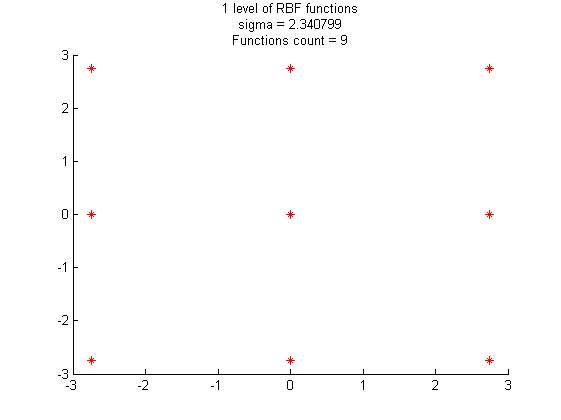
\includegraphics[width=0.33\textwidth]
	{images/centers1.png}}
	\subfloat
	{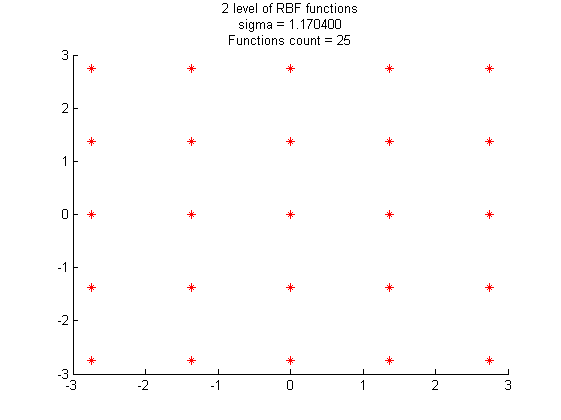
\includegraphics[width=0.33\textwidth]
	{images/centers2.png}}
	\subfloat
	{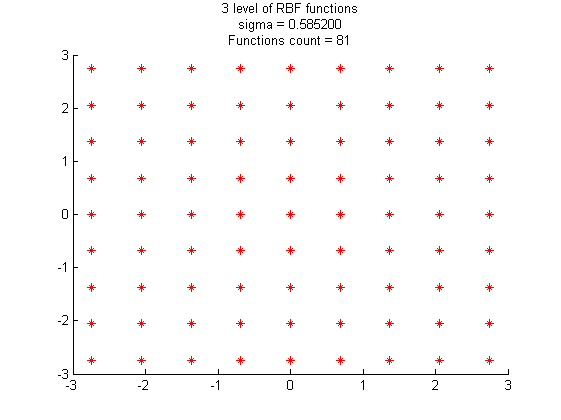
\includegraphics[width=0.33\textwidth]
	{images/centers3.png}}

	\caption{Centra wygenerowanych funkcji RBF}
	\label{img:rbf_centers}
\end{figure}

Następnie dokonano selekcji najbardziej istotnych funkcji z biblioteki wykorzystując metodę GOFR. Po selekcji każdej z funkcji dokonywana jest optymalizacja wybranej funkcji metodą Levenberga-Marquardta. Sieć neuronowa o funkcjach bazowych zdefiniowanych wzorem \ref{wzor:rbf_2d} realizuje funkcję:
\begin{equation}
	\tilde{y} = \sum_{i=1}^N w_i f_i(x_1,x_2,c_1,c_2,\sigma_i)
\end{equation}
Optymalizowano następujące parametry sieci RBF: $c_1$, $c_2$, $\sigma$ oraz $w$. Zgodnie z omówioną w rodziale \ref{rozdzial:l-m} konieczne jest określenie gradientu funkcji błędu $e = y - \tilde{y}$. Funkcja błędu $e$ jest wyrażona wzorem:
\begin{equation}
	e = y - \tilde{y} = y - w f(x_1,x_2,c_1,c_2,\sigma) = y - w e^{-\frac{(x_1-c_1)^2 + (x_2-c_2)^2}{2 \sigma^2}} 
\end{equation}
Gradient $e$ wynosi zatem:
\begin{equation}
\begin{bmatrix}
	\frac{\partial e}{\partial w} \\
	\frac{\partial e}{\partial \sigma} \\
	\frac{\partial e}{\partial c_1} \\
	\frac{\partial e}{\partial c_2}
\end{bmatrix} = 
\begin{bmatrix}
	f(\cdot) \\
	w f(\cdot) \frac{(x_1 - c_1)^2 + (x_2 - c_2)^2}{\sigma^3}\\
	w f(\cdot) \frac{(x_1 - c_1)}{\sigma^2}\\
	w f(\cdot) \frac{(x_2 - c_2)}{\sigma^2}	
\end{bmatrix}
\end{equation}

W przypadku zwiększania się błędu $\lambda$ ze wzoru \ref{wzor:mse_lm} była zwiększana 10-krotnie, w przypadku zmniejszania się błędu $\lambda$ była zmniejszana 10-krotnie. Warunek stopu został ustalony tak aby błąd średniokwadratowy dla każdego z wyjść z sieci był mniejszy od 1e-5. Schemat sieci użytej do rozwiązania równania Van der Pola przedstawia rysunek \ref{fig:rbf}.

\begin{figure}[ht!]
	\centering
	
	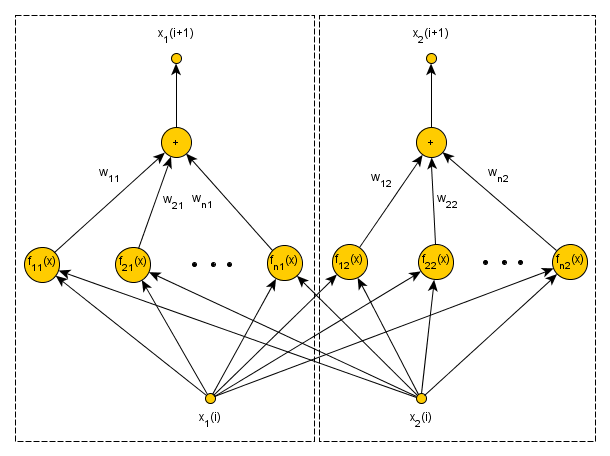
\includegraphics[width = \textwidth]{images/rbf.png}
	\caption{Schemat zaprojektowanej sieci RBF}
	\label{fig:rbf}	

\end{figure}


\clearpage
\section{Wyniki identyfikacji systemu opisanego równaniem Van der Pola}

Osiągnięcie błędu średniokwadratowego poniżej 1e-5 udało się osiągnąć dla 13 funkcji bazowych dla funkcji $y(t)$ (błąd równy = 1.7227e-6) oraz 18 funkcji bazowych dla pochodnej $y'(t)$ (błąd równy = 8.9721e-6). Na rysunku \ref{fig:aproksymacja_x1} oraz rysunku \ref{fig:aproksymacja_x2} zostały przedstawione odpowiednio: aproksymacja w kolejnych iteracjach funkcji $y(t)$ równania Van der Pola oraz aproksymacja pierwszej pochodnej $y'(t)$ dla pierwszych sześciu iteracji. Na rysunku \ref{img:approximated} została przedstawiona aproksymacja równania Van der Pola przez wytrenowaną sieć.

\begin{figure}[ht!]
	\centering
	
	\subfloat
	{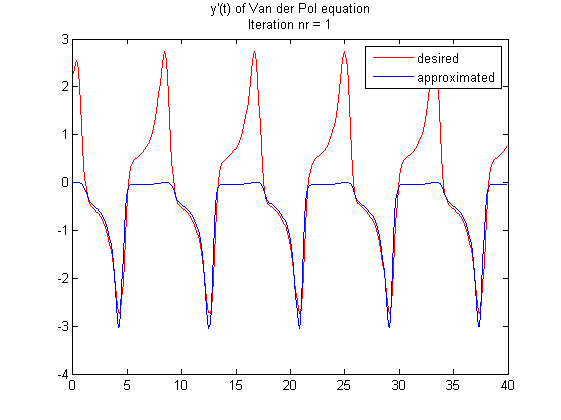
\includegraphics[width=0.5\textwidth]
	{images/deriv_iter1.png}}
	\subfloat
	{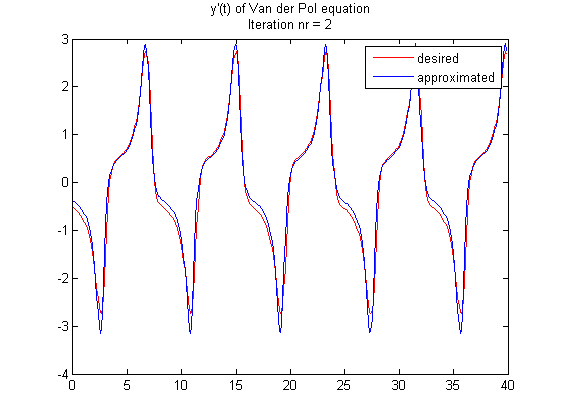
\includegraphics[width=0.5\textwidth]
	{images/deriv_iter2.png}}
	
	\subfloat
	{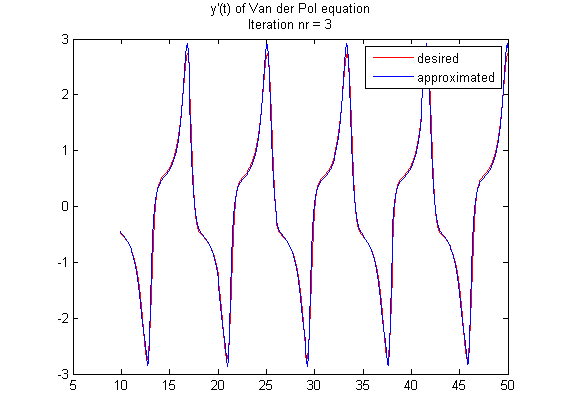
\includegraphics[width=0.5\textwidth]
	{images/deriv_iter3.png}}
	\subfloat
	{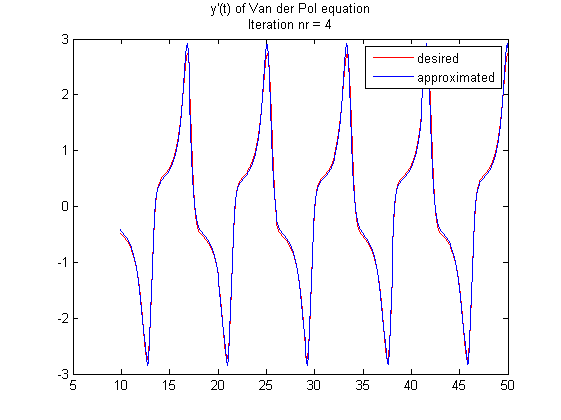
\includegraphics[width=0.5\textwidth]
	{images/deriv_iter4.png}}

	\subfloat
	{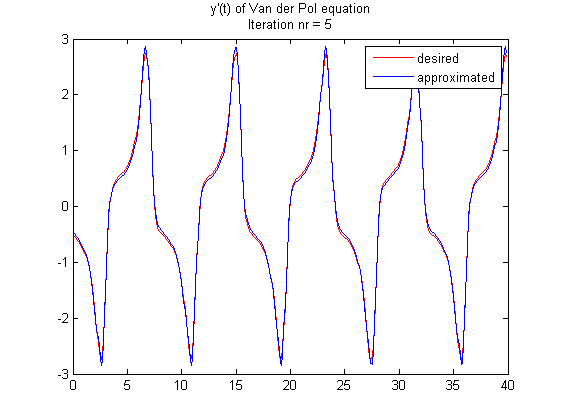
\includegraphics[width=0.5\textwidth]
	{images/deriv_iter5.png}}
	\subfloat
	{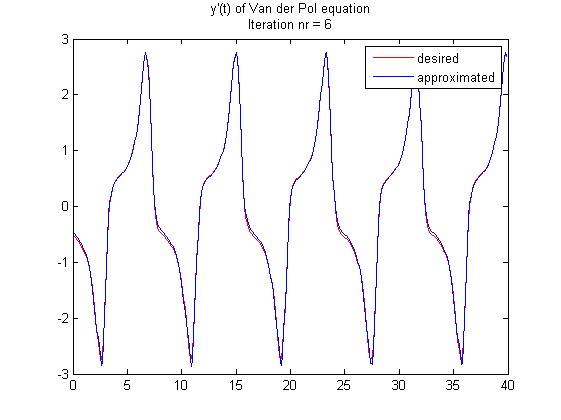
\includegraphics[width=0.5\textwidth]
	{images/deriv_iter6.png}}	
	
	\caption{Aproksymacja funkcji y(t)}		
	\label{fig:aproksymacja_x1}
\end{figure}


\begin{figure}[ht!]
	\centering

	\subfloat
	{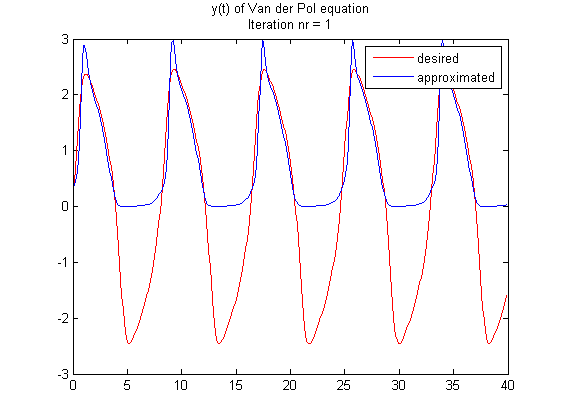
\includegraphics[width=0.5\textwidth]
	{images/signal_iter1.png}}
	\subfloat
	{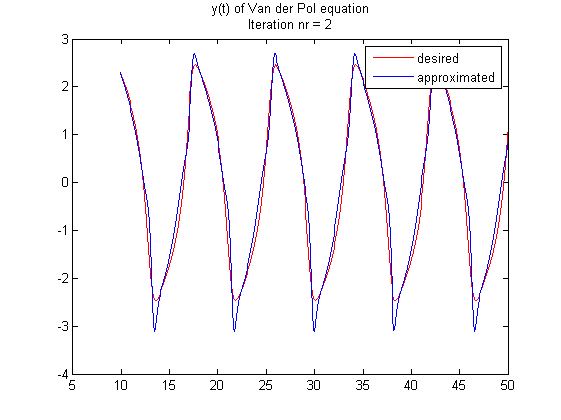
\includegraphics[width=0.5\textwidth]
	{images/signal_iter2.png}}
	
	\subfloat
	{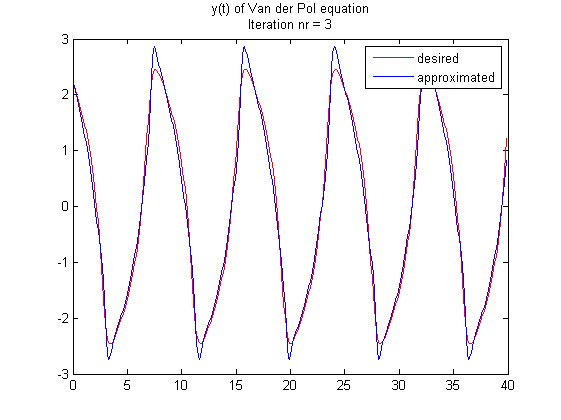
\includegraphics[width=0.5\textwidth]
	{images/signal_iter3.png}}
	\subfloat
	{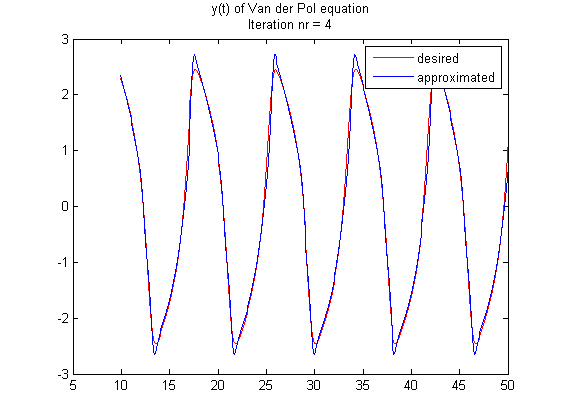
\includegraphics[width=0.5\textwidth]
	{images/signal_iter4.png}}

	\subfloat
	{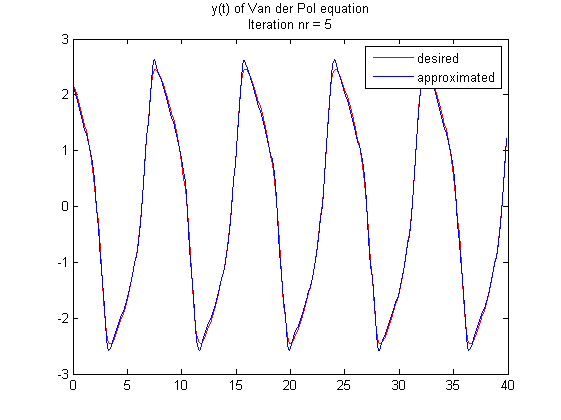
\includegraphics[width=0.5\textwidth]
	{images/signal_iter5.png}}
	\subfloat
	{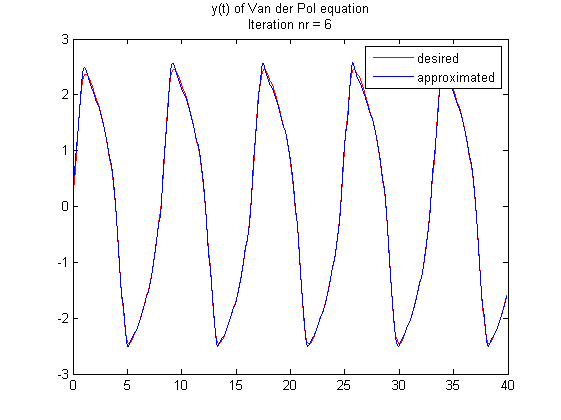
\includegraphics[width=0.5\textwidth]
	{images/signal_iter6.png}}	

	\caption{Aproksymacja funkcji y'(t)}		
	\label{fig:aproksymacja_x2}		
\end{figure}


\begin{figure}[ht!]
	\centering

	\subfloat
	{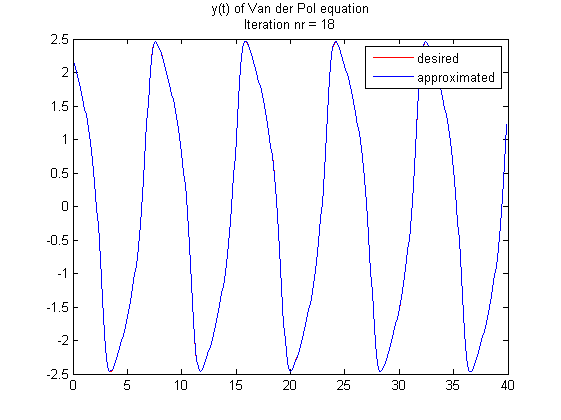
\includegraphics[width=0.5\textwidth]
	{images/signal_approx.png}}
	\subfloat
	{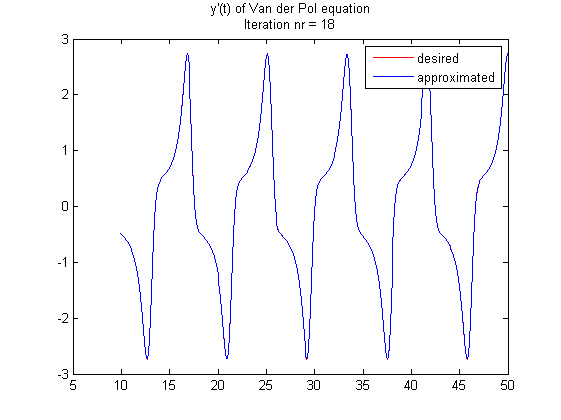
\includegraphics[width=0.5\textwidth]
	{images/deriv_approx.png}}	
	
	\subfloat
	{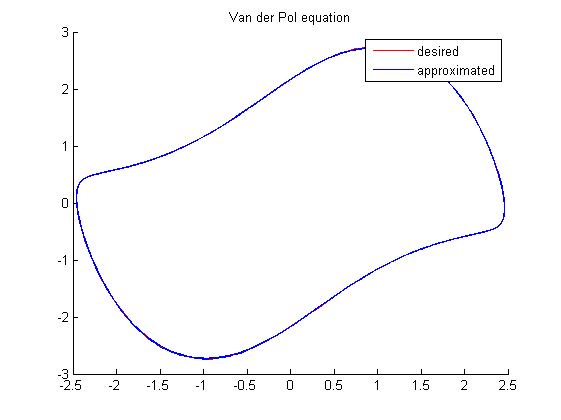
\includegraphics[width=0.5\textwidth]
	{images/trajectory_approx.png}}

	\caption{Sygnał zadany oraz aproksymowany przez wytrenowaną sieć RBF $t \in [0,50]$}
	\label{img:approximated}
\end{figure}


W tabeli \ref{tab:rbf_tabela_x1} zostały zebrane dane na temat wybranych funkcji RBF oraz błąd średniokwadratowy aproksymacji funkcji $y(t)$ równania Van der Pola po selekcji kolejnych funkcji RBF.
\begin{table}[ht!]
\centering

\begin{tabular}{ |c| c| c| c| c| c| }
\hline
Indeks RBF & centrum 1 & centrum 2 & szerokość $\sigma$ & energia      & błąd MSE \\ \hline    
	
	12     &  -3.1410  & -0.7327   &  1.5642            & 4.9705e-001  & 1.4668e+000 \\
     8     &   5.4244  &  0.9766   &  2.5508            & 4.7447e-001  & 8.3072e-002 \\
     2     &  -7.7925  & -1.6129   &  4.0497            & 1.5925e-002  & 3.6628e-002 \\
    98     &   2.2304  & -3.0565   &  0.7112            & 6.0098e-003  & 1.9101e-002 \\
    29     &   1.0666  &  3.0337   &  1.0207            & 4.9036e-003  & 4.8007e-003 \\
     7     &   1.7472  & -1.5353   &  1.9623            & 9.6393e-004  & 1.9895e-003 \\
     9     &   3.8354  &  3.6792   &  2.7580            & 4.2284e-004  & 7.5638e-004 \\
    41     &  -2.4850  &  0.9208   &  0.6385            & 1.3605e-004  & 3.5963e-004 \\
    27     &   1.2187  &  0.1897   &  1.0115            & 8.3280e-005  & 1.1675e-004 \\
    30     &   2.6590  & -2.6077   &  1.1867            & 2.6429e-005  & 3.9676e-005 \\
    36     &  -2.8032  & -2.0897   &  0.6533            & 6.0339e-006  & 2.2079e-005 \\
    88     &   0.7563  &  2.3091   &  0.4725            & 3.3734e-006  & 1.2241e-005 \\
    76	   &   0.1031  &  0.7697   &  0.5688            & 3.6066e-006  & 1.7227e-006 \\
    \hline
\end{tabular}

\caption{Wybrane funkcje RBF dla y(t)}
\label{tab:rbf_tabela_x1}
\end{table}

W tabeli \ref{tab:rbf_tabela_x2} zostały zebrane dane na temat wybranych funkcji RBF oraz błąd średniokwadratowy aproksymacji pochodnej $y'(t)$ równania Van der Pola po selekcji kolejnych funkcji RBF.

\begin{table}[ht!]
\centering

\begin{tabular}{ |c| c| c| c| c| c| }
\hline
Indeks RBF & centrum 1 & centrum 2 & szerokość $\sigma$ & energia      & błąd MSE    \\ \hline    
    20     &  1.1527   &  -5.6961  &       2.0452       &  4.8649e-001 & 9.7293e-001 \\
    24     & -0.6262   &   5.0882  &       2.1711       &  4.9361e-001 & 3.7704e-002 \\
    71     &  0.4140   &  -3.5549  &       0.8248       &  1.1321e-002 & 1.6255e-002 \\
    55     & -1.4563   &  -1.3841  &       0.6117       &  4.7338e-003 & 7.2860e-003 \\
   105     &  2.8298   &   2.3938  &       0.7238       &  1.9506e-003 & 3.5903e-003 \\
    87     &  0.4339   &   2.4652  &       0.6929       &  9.2016e-004 & 1.8469e-003 \\
    31     &  2.7273   &  -1.5110  &       1.1974       &  5.1159e-004 & 8.7764e-004 \\
    35     & -2.4111   &  -2.8130  &       0.3998       &  1.7996e-004 & 5.3668e-004 \\
    37     & -3.3572   &  -1.5420  &       0.7056       &  8.9771e-005 & 3.6660e-004 \\
    62     & -0.6001   &  -3.3387  &       0.4237       &  7.7115e-005 & 2.2049e-004 \\
    72     & -0.0875   &  -1.9432  &       0.5984       &  2.3360e-005 & 1.7624e-004 \\
    34     &  2.2615   &   2.2518  &       1.0292       &  1.7416e-005 & 1.4324e-004 \\
   108     &  2.8108   &  -2.1227  &       0.5800       &  1.4040e-005 & 1.1664e-004 \\
    79     &  0.1036   &   2.5772  &       0.5447       &  2.3562e-005 & 7.1994e-005 \\
    46     & -1.9407   &  -1.3306  &       0.5779       &  1.3514e-005 & 4.6389e-005 \\
    39     & -3.6363   &   0.1453  &       0.7197       &  1.4067e-005 & 1.9737e-005 \\
     8     &  2.7351   &   0.0047  &       2.3403       &  4.4026e-006 & 1.1395e-005 \\
    73     & -0.0697   &  -1.2975  &       0.5822       &  1.2790e-006 & 8.9721e-006 \\
    \hline
\end{tabular}

\caption{Wybrane funkcje RBF dla y'(t)}
\label{tab:rbf_tabela_x2}
\end{table}

\clearpage

Po etapie trenowania sieci RBF sprawdzono zdolność tej sieci do predykcji. Predykcja na 100 kroków do przodu została przedstawiona na rysunku~\ref{img:predicted}. Jak można zauważyć sieć jest zdolna do predykcji równania Van der Pola. Błąd średniokwadratowy dla wyznaczania $y(t)$ wyniósł 0.0085, natomiast błąd predykcji wyznaczania $y'(t)$ wyniósł  4.9856.

\begin{figure}[ht!]
	\centering

	\subfloat
	{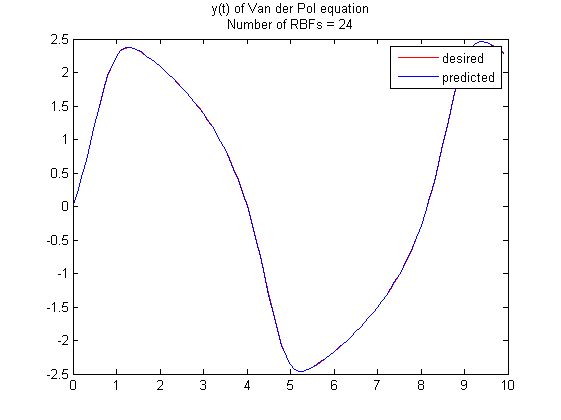
\includegraphics[width=0.5\textwidth]
	{images/signal_pred100.png}}
	\subfloat
	{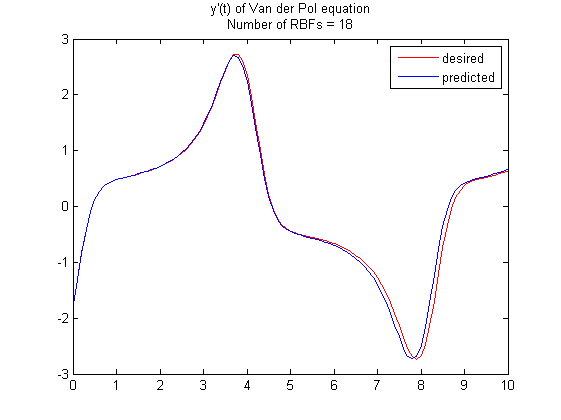
\includegraphics[width=0.5\textwidth]
	{images/deriv_pred100.png}}	
	
	\subfloat
	{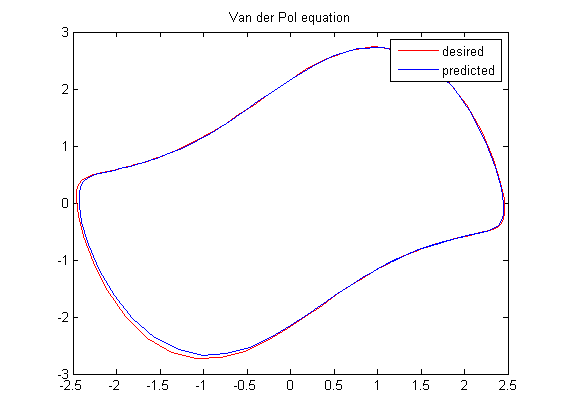
\includegraphics[width=0.5\textwidth]
	{images/trajectory_pred100.png}}

	\caption{Sygnał zadany oraz przewidywany przez wytrenowaną sieć RBF $t \in [0,10]$}
	\label{img:predicted}
\end{figure}


Na rysunku \ref{img:err} został przedstawiony błąd w funkcji $t$.

\begin{figure}[ht!]
	\centering

	\subfloat
	{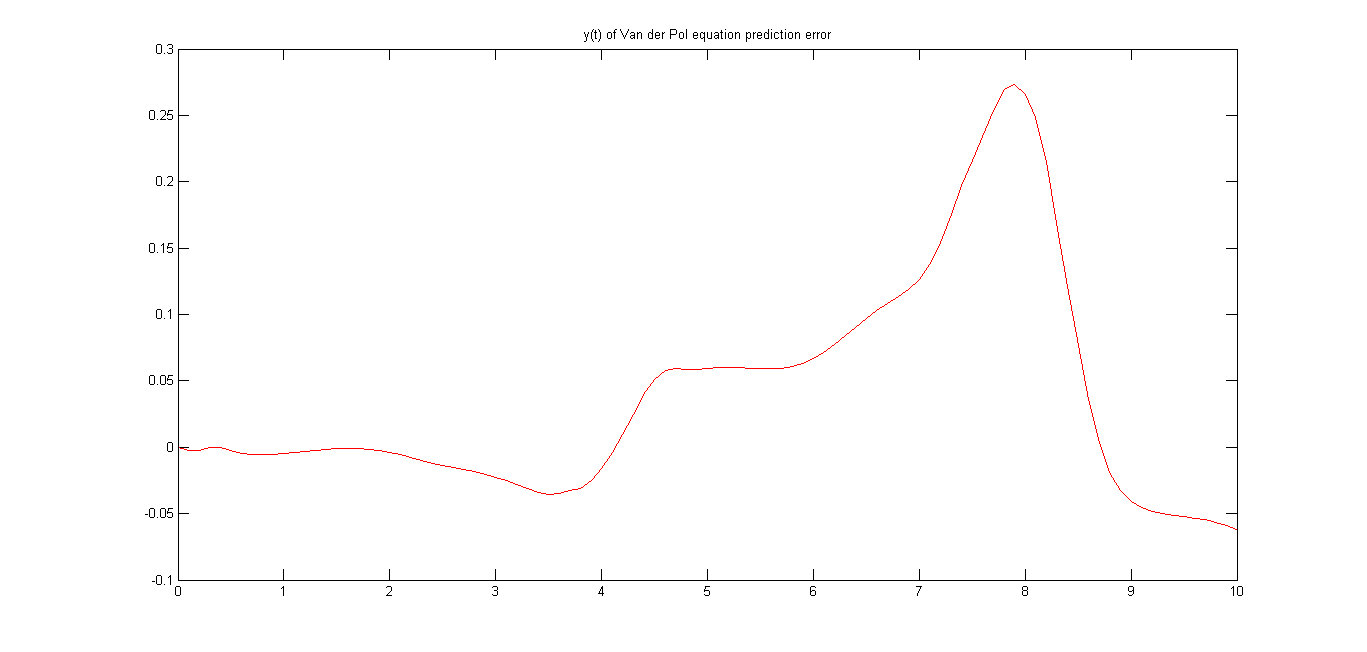
\includegraphics[width=0.5\textwidth]
	{images/err100_x1.png}}
	\subfloat
	{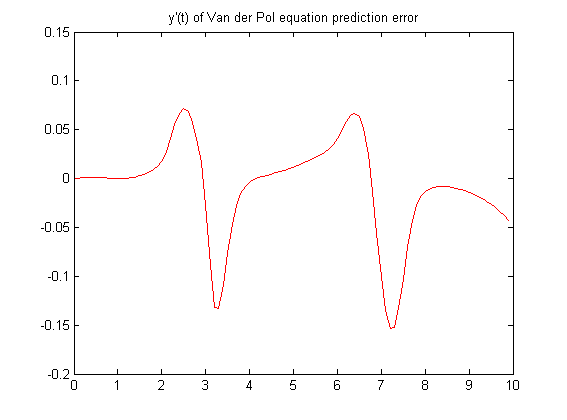
\includegraphics[width=0.5\textwidth]
	{images/err100_x2.png}}	
	

	\caption{Błąd predykcji w funkcji czasu $t \in [0,10]$}
	\label{img:err}
\end{figure}


Na rysunku \ref{img:predicted2} została przedstawiana predykcja w szerszym przedziale czasu. Jak można zauważyć predykcja z biegiem czasu zaczyna coraz bardziej odstępować od wartości oczekiwanej.

\begin{figure}[ht!]
	\centering

	\subfloat
	{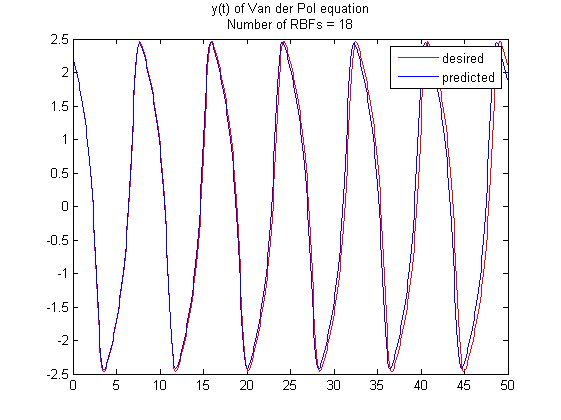
\includegraphics[width=0.5\textwidth]
	{images/signal_pred400.png}}
	\subfloat
	{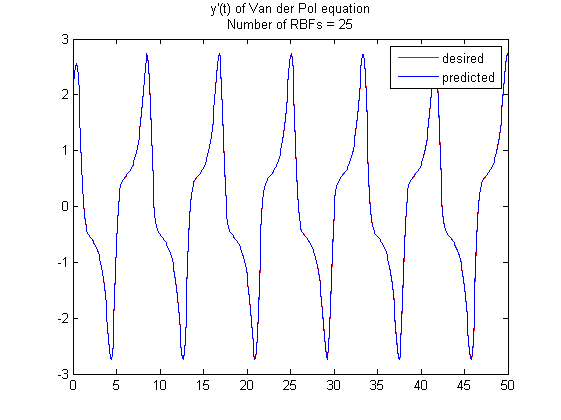
\includegraphics[width=0.5\textwidth]
	{images/deriv_pred400.png}}	
	
	\subfloat
	{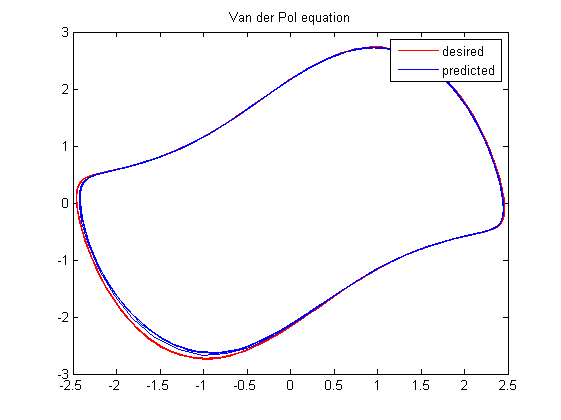
\includegraphics[width=0.5\textwidth]
	{images/trajectory_pred400.png}}

	\caption{Sygnał zadany oraz przewidywany przez wytrenowaną sieć RBF $t \in [0,40]$}
	\label{img:predicted2}
\end{figure}



\clearpage
\section{Podsumowanie oraz wnioski}
Celem pracy była próba identyfikacji nieliniowych obiektów dynamicznych z wykorzystaniem metody GOFR. Cel udało się zrealizować identyfikując obiekt dynamiczny opisany równaniem Van der Pola. Predykcja działała na ponad kilkadziesiąt kroków w przód. Można jednak zauważyć, że predykcja wraz ze wzrostem czasu pogarszała się. Dzieje się tak ze względu na akumulacje błędów predykcji wraz ze wzrostem czasu. Kolejną wadą zidentyfikowanego modelu jest fakt identyfikacji tylko dla wcześniej określonego kroku. Należy jednak podkreślić, że pomimo tych wad model dobrze spełnia swoje zadanie.


% -------------------------- bibliografia ----------------------------
\clearpage

\addcontentsline{toc}{section}{Literatura}
\begin{thebibliography}{widest-label}

\bibitem{AK_RBG2002}Kharab A., Ronald B. Guenther, An introduction to numerical methods : a MATLAB approach, 2002, Chapman \& Hall/CRC

\bibitem{BCh_2001}Bogdan Choczewski (red.), Równania różniczkowe zwyczajne i cząstkowe. Zadania z matematyki, Kraków 2001, Wydawnictwa AGH

\bibitem{Osowski}Osowski S., Sieci neuronowe do przetwarzania informacji, Warszawa 2006, Oficyna Wydawnicza Politechniki Warszawskiej

\bibitem{Bishop}Bishop C. M., Neural Networks for Pattern Recognition, Oxford University Press, 1995 Oxford

\bibitem{Bartkowiak} Bartkowiak A., (Notatki do wykładu Sieci Neuronowe), Sieci RBF - o radialnych funkcjach bazowych, https://www.ii.uni.wroc.pl/~aba/teach/NN/w9rbf.pdf

\bibitem{Chen} Chen S., Cowan C. F. N., Grant P. M., Orthogonal Least Squares Learning Algorithm for Radial Basis Function Networks, IEEE, 1991

\bibitem{Duboisa} R. Duboisa, B. Queneta, Y. Faisandierb, G. Dreyfusa, Building meaningful representations for nonlinear modeling of 1d- and 2d-signals: applications to biomedical signals

\bibitem{Gutenbaum} J. Gutenbaum, Modelowanie systemów,

\bibitem{Kosinski} R. A. Kosiński, Sztuczne sieci neuronowe, Warszawa 2007, WNT
\end{thebibliography}

\clearpage
\addcontentsline{toc}{section}{Dodatek A: Kod źródłowy programu}
\section*{Dodatek A: Kod źródłowy programu}

\textit{van\_der\_pol.m}

\begin{lstlisting}
% Function solving Van der Pol equations usign 4-th order Runge-Kutta method
%
% t_end - end of time period for solution (time starts from 0)
% h     - time step
% y0    - init values

function [t,y] = rk_van_der_pol(t_end, h, y0)

    % Runge-Kutta general formula
    % y_{i+1} = y_i + 1/6*(k_1 + 2k_2 + 2k_3 + k_4), i = 0,1,2,...
    % k_1 = hf(x_i,y_1)
    % k_2 = hf(x_i + 1/2h, y_1 + 1/2k_1)
    % k_3 = hf(x_i + 1/2h, y_1 + 1/2k_2)    
    % k_4 = hf(x_i + h, y_1 + k_3)
    
    t = 0:h:t_end;
    n = length(t);
    h = 0.1;

    y = zeros(n, 2);
    y(1, 1) = y0(1);
    y(1, 2) = y0(2);
    
    % Van der Pol equation 
    % y''(t) - (1 - y^2(t)) * y'(t) + y(t) = 0;
    % y'(t)  = y(2)
    % y''(t) = (1-y(1)^2)*y(2)-y(1)

    for i = 1:n-1
        k1 = h*(y(i,2));
        k2 = h*(y(i,2)+0.5*k1);
        k3 = h*(y(i,2)+0.5*k2);
        k4 = h*(y(i,2)+k3);
        y(i+1,1) = y(i,1)+(k1+2*k2+2*k3+k4)/6;
        
        y1 = y(i,1);
        y2 = y(i,2);
        k1 = h*((1-y1^2)*y2-y1);
        y1 = y(i,1)+0.5*k1;
        y2 = y(i,2)+0.5*k1;
        k2 = h*((1-y1^2)*y2-y1);
        y1 = y(i,1)+0.5*k2;
        y2 = y(i,2)+0.5*k2;
        k3 = h*((1-y1^2)*y2-y1);
        y1 = y(i,1)+k3;
        y2 = y(i,2)+k3;
        k4 = h*((1-y1^2)*y2-y1);
        y(i+1,2) = y(i,2)+(k1+2*k2+2*k3+k4)/6;

    end
    
end

\end{lstlisting}

\textit{gofr.m}

\begin{lstlisting}
function [selected_rbfs, W, E_k, A_k, Q_k, B_k, centers, sigmas, G] =  gofr(X, y, G, centers, sigmas, K)

    rbf_number = length(centers);

    % TODO: comment these variables
    D = y;
    Q = zeros(size(G));
    Q_k = zeros(size(G));
    B = zeros(1,rbf_number);
    B_k = zeros(1,rbf_number);
    E = zeros(1,rbf_number);
    E_k = zeros(1,K);
    selected_rbfs = zeros(1,rbf_number);      % indexes of selected rbfs order by decreasing energy 

    A = cell(1,rbf_number);
    A_k = eye(rbf_number);
    for i = 1:rbf_number
        A{i} = eye(rbf_number);
    end

    % ----- selection of the most significant functions -----
    for k = 1:K
        % Gram-Schmidt orthogonalization
        for i = 1:rbf_number
           Q(:,i) = G(:,i);

           % if rbf is already selected function omit it 
           if ismember(i, selected_rbfs) == 1
               continue;
           end

           for j=1:k-1
                A{i}(j,k) = Q_k(:,j)'*G(:,i) / (Q_k(:,j)'*Q_k(:,j));
                Q(:,i) = Q(:,i) - A{i}(j,k)*Q_k(:,j);
           end

           B(i) = Q(:,i)'*D / (Q(:,i)'*Q(:,i));
           E(i) = B(i)^2*Q(:,i)'*Q(:,i) / (D'*D);   
        end

        % find RBF with maximum energy (save index and copy to Q_k matrix)
        [E_k(k) selected_rbfs(k)] = max(E);
        B_k(k) = B(selected_rbfs(k));
        A_k(:,k) = A{selected_rbfs(k)}(:,k);
        W = A_k\B_k';

        % ------ Levenberg-Marquardt -----
        Theta = [W(k); sigmas(selected_rbfs(k)); centers(1, selected_rbfs(k)); centers(2, selected_rbfs(k))];

        y_rbf = 0;
        for j = 1:k
            y_rbf = y_rbf + W(j) * gaussian_2D(X, sigmas(selected_rbfs(j)), centers(:,selected_rbfs(j))');
        end
        

        lambda = 0.1;
        Theta_old = Theta;
        N = 100;   % maximum iterations of gradient method
        err = zeros(N,1);
        err(1) = abs(sum((y - y_rbf).^2)) / length(y);
        err_old = err(1);
        for n = 2:N
          
            dy_dw = gaussian_2d(X, Theta(2), [Theta(3) Theta(4)]);
            dy_dsigma = Theta(1) * ((Theta(3) - X(:,1)).^2 + (Theta(4) - X(:,2)).^2) ./ (Theta(2)^3) .* gaussian_2d(X, Theta(2), [Theta(3) Theta(4)]);
            dy_dc1 = (Theta(1)*(X(:,1) - Theta(3))) ./ (Theta(2)^2) .* gaussian_2d(X, Theta(2), [Theta(3) Theta(4)]);
            dy_dc2 = (Theta(1)*(X(:,2) - Theta(4))) ./ (Theta(2)^2) .* gaussian_2d(X, Theta(2), [Theta(3) Theta(4)]);
            
            Z = [dy_dw dy_dsigma dy_dc1 dy_dc2];
            e = y - y_rbf;

            Theta = Theta + pinv(Z'*Z + lambda*eye(4))*Z'*e;            
            W(k) = Theta(1);
            sigmas(selected_rbfs(k)) = Theta(2);
            centers(1,selected_rbfs(k)) = Theta(3);
            centers(2,selected_rbfs(k)) = Theta(4);
            
            y_rbf = 0;
            for j = 1:k
                y_rbf = y_rbf + W(j) * gaussian_2D(X, sigmas(selected_rbfs(j)), centers(:,selected_rbfs(j))');
            end

            err(n) = sum((y - y_rbf).^2) / length(y);
            if (err(n) >= err_old)
                Theta = Theta_old;
                lambda = lambda * 10;
            else
                Theta_old = Theta;
                err_old = err(n);
                lambda = lambda / 10;                
            end

            % if lambda is too big or too small stop
            if (lambda > 1e6 || lambda < 1e-6)
                break;
            end;
            
            if (err(n) < 1e-6)
                break;
            end
        end;
        
        % set the optimal parameters
        W(k) = Theta_old(1);
        sigmas(selected_rbfs(k)) = Theta_old(2);
        centers(1,selected_rbfs(k)) = Theta_old(3);
        centers(2,selected_rbfs(k)) = Theta_old(4);

        % Gram-Schmidt orthogonalization for modified RBF
        i = selected_rbfs(k);
        G(:,i) = gaussian_2D(X, Theta(2), [Theta(3) Theta(4)]);
        Q(:,i) = G(:,i);

        for j=1:k-1
            A{i}(j,k) = Q_k(:,j)'*G(:,i) / (Q_k(:,j)'*Q_k(:,j));
            Q(:,i) = Q(:,i) - A{i}(j,k)*Q_k(:,j);
        end

        B(i) = Q(:,i)'*D / (Q(:,i)'*Q(:,i));
        B_k(k) = B(i);
        E_k(k) = B(i)^2*Q(:,i)'*Q(:,i) / (D'*D);
        A_k(:,k) = A{i}(:,k);
        Q_k(:,k) = Q(:,i);

        W = A_k\B_k';

        E = zeros(size(E));
    end

    W = A_k\B_k';

end
\end{lstlisting}

\textit{generate\_library\_2d.m}

\begin{lstlisting}
% ----- Function generating radial basis function set -----
% N - number of dividing set iteration - change this variable if want other number of RBFs
% G - matrix with values of all rbf functions
% centers - vector of centers of all rbf functions
% sigmas - vector of sigma of all rbf functions

function [G,centers,sigmas] = generate_library_2d(X, N)

    rbf_number = 0; % total number of RBFs

    for i = 1:N
        rbf_number = rbf_number + (2^i + 1)^2;
    end

    G = zeros(length(X), rbf_number);
    centers = zeros(2, rbf_number);
    sigmas = zeros(1, rbf_number);
    k = 1;

    max_x = max(max(X));
    min_x = min(min(X));

    for i = 1:N

        iter_rbf_count = 2^i+1;  % number of RBFs in current iteration
        sigma = sqrt(max_x - min_x) / 2^(i-1);

    %     figure(i+1)
    %     title({sprintf('%d level of RBF functions',i);
    %            sprintf('sigma = %f',sigma);
    %            sprintf('Functions count = %d',iter_rbf_count^2)})
    %     hold on

        for j = 1:iter_rbf_count
            % generating centers for rbf functions
            for l = 1:iter_rbf_count
                centers(1, k) = min_x + (max_x - min_x) / (iter_rbf_count-1) * (j-1);
                centers(2, k) = min_x + (max_x - min_x) / (iter_rbf_count-1) * (l-1);
                G(:,k) = gaussian_2d(X, sigma, centers(:,k)'); 
    %             plot(centers(1,k),centers(2,k),'r*');
                sigmas(k) = sigma;
                k = k + 1;
            end
        end    

    %     hold off;
    end

end
\end{lstlisting}

\textit{gofr\_van\_der\_pol.m}

\begin{lstlisting}
% Neural network with radial basis functions (RBF) approximating 
% Van der Pol equation using Orthogonal Forward Regression (OFR)

close all;
clear all;
clc;

% ----- generating training data -----
[t Y] = rk_van_der_pol(50, 0.1, [0 2]);
X(:,1) = Y(99:end-1,1);
X(:,2) = Y(99:end-1,2);
y1 = Y(100:end,1);
y2 = Y(100:end,2);

% ----- generating radial basis function set -----
N = 3;

% ----- teach RBF neural network -----
for K1 = 1:30
    K1
    [G1 centers1 sigmas1] = generate_library_2d(X, N);
    [selected_rbfs1, W1, E_k1, A_k1, Q_k1, B_k1, centers1, sigmas1, G1] =  gofr(X, y1, G1, centers1, sigmas1, K1);
    y_rbf1 = 0;
    for i = 1:K1
        y_rbf1 = y_rbf1 + W1(i) * G1(:,selected_rbfs1(i));
    end
    err(K1,1) = sum((y1 - y_rbf1).^2) / length(y1);
    
    if (err(K1,1) < 1e-5)
        break;
    end
end

for K2 = 1:30
    K2
    [G2 centers2 sigmas2] = generate_library_2d(X, N);
    [selected_rbfs2, W2, E_k2, A_k2, Q_k2, B_k2, centers2, sigmas2, G2] =  gofr(X, y2, G2, centers2, sigmas2, K2);
    y_rbf2 = 0;
    for i = 1:K2
        y_rbf2 = y_rbf2 + W2(i) * G2(:,selected_rbfs2(i));
    %     y_rbf2 = y_rbf2 + W2(i) * gaussian_2D(X, sigmas2(selected_rbfs2(i)), centers2(:,selected_rbfs2(i))');
    end
    err(K2,2) = sum((y2 - y_rbf2).^2) / length(y2);

    if (err(K2,2) < 1e-5)
        break;
    end

end

% ----- function approximation by RBF neural network -----


figure(1)
plot(t(100:end), y1, 'r', t(100:end), y_rbf1, 'b');
title('y(t) of Van der Pol equation');
legend('desired','approximated');

figure(2)
plot(t(100:end), y2, 'r', t(100:end), y_rbf2, 'b');
title('y''(t) of Van der Pol equation');
legend('desired','approximated');

figure(3)
hold on;
plot(y1, y2, 'r', y_rbf1, y_rbf2, 'b');
title('Van der Pol equation');
legend('desired','approximated');


% ----- function predictioin by RBF neural network -----
P = 500;        % prediction steps
y_rbf1 = zeros(1,P);
y_rbf2 = zeros(1,P);
% y_rbf1(1) = y1(200);
% y_rbf2(1) = y2(200);
y_rbf1(1) = 0.1;
y_rbf2(1) = -3;
[t Y] = rk_van_der_pol(P*0.1-0.1, 0.1, [y_rbf1(1) y_rbf2(1)]);
y1 = Y(100:end,1);
y2 = Y(100:end,2);

y_rbf1(1) = y1(1);
y_rbf2(1) = y2(1);

for j = 2:P
    for i = 1:K1
        y_rbf1(j) = y_rbf1(j) + W1(i) * gaussian_2D([y_rbf1(j-1) y_rbf2(j-1)], sigmas1(selected_rbfs1(i)), centers1(:,selected_rbfs1(i))');
    end
    
    for i = 1:K2
        y_rbf2(j) = y_rbf2(j) + W2(i) * gaussian_2D([y_rbf1(j-1) y_rbf2(j-1)], sigmas2(selected_rbfs2(i)), centers2(:,selected_rbfs2(i))');        
    end
end

figure(4)
plot(t(1:end-99),y1,'r', t(1:end-99) ,y_rbf1(1:end-99),'b');
title({'y(t) of Van der Pol equation'; sprintf('Number of RBFs = %d', K1)});
legend('desired','predicted');

rms1 = sqrt(sum((y_rbf1(1:end-99)' - y1).^2) / length(y1));

figure(5)
plot(t(1:end-99),y2,'r', t(1:end-99) ,y_rbf2(1:end-99),'b');
title({'y''(t) of Van der Pol equation'; sprintf('Number of RBFs = %d', K2)});
legend('desired','predicted');

rms2 = sqrt(sum((y_rbf1(1:end-99)' - y2).^2) / length(y2));
\end{lstlisting}

\end{document}
